\documentclass[11pt]{article}

\usepackage[T1]{fontenc}
\usepackage{lmodern}
\usepackage[margin=1in]{geometry}
\usepackage{amsmath,amssymb,mathtools}
\usepackage{array}
\usepackage{booktabs}
\usepackage{graphicx}
\usepackage{tikz}
\usetikzlibrary{arrows.meta,positioning}
\usepackage{microtype}
\usepackage{xcolor}
\usepackage[hidelinks]{hyperref}

\definecolor{MSSNavy}{HTML}{12304A}
\definecolor{MSSOrange}{HTML}{D96B1B}

\newcommand{\matM}{\bar M}
\newcommand{\code}[1]{\texttt{#1}}

% All worked-example values are computed by Python. Do not type them here.
\input{../Presentation/generated/unveiling_values.tex}
\input{../Presentation/generated/figure1_values.tex}
\input{../Presentation/generated/figure1_authors_values.tex}

\title{Replication Report: Financial-Network Unveiling}
\author{Course replication exercise}
\date{\today}

\begin{document}

\maketitle

\section{The Leontief unveiling operator}
\label{sec:leontief}

\subsection{Economic object and notation}

Mian, Straub, and Sufi (2025, Sections 2.1--2.2) ask who ultimately owns a
financial claim when the observed holder is itself a financial intermediary.
Let $\matM_t$ denote the direct ownership matrix. Its entry $\matM_t(i,j)$ is
the share of sector $i$'s liabilities held directly by sector $j$. Rows are
therefore issuers or borrowers, columns are holders or lenders, and every row
sums to one.

This normalization is row-specific. For example, the outgoing entries from a
bank all divide by that bank's total liabilities, so they describe who funds
the bank and sum to one. An incoming entry such as $\matM_t(F,B)=0.20$ instead
says that the bank holds 20 percent of fund $F$'s liabilities; its denominator
is $F$'s liabilities, not the bank's assets. Columns therefore need not sum to
one. Intermediaries do own assets directly, but they are not terminal owners:
their assets are financed by liabilities and equity that are themselves held
by other sectors.

Order the $m$ ultimate owners before the $k$ intermediaries. After zeroing the
owner rows, the matrix relevant for intermediation has block form

\begin{equation}
  M_t=
  \begin{bmatrix}
    0   & 0   \\
    B_t & Q_t
  \end{bmatrix},
\end{equation}

where $B_t\in\mathbb{R}^{k\times m}$ contains intermediaries' direct owner
shares and $Q_t\in\mathbb{R}^{k\times k}$ contains intermediary
cross-holdings. The paper writes the sum over all ownership paths as

\begin{equation}
  \bar\Omega_t=M_t+M_t^2+M_t^3+\cdots=M_t(I-M_t)^{-1}.
  \label{eq:paper-leontief}
\end{equation}

The lower-left block is the required ultimate-ownership matrix,

\begin{equation}
  \Omega_t
  =B_t+Q_tB_t+Q_t^2B_t+\cdots
  =(I-Q_t)^{-1}B_t.
  \label{eq:block-leontief}
\end{equation}

The maintained condition $\rho(Q_t)<1$ ensures that intermediary
cross-holdings eventually reach an ultimate owner. Economically, the network
cannot contain a closed group of intermediaries that own 100 percent of one
another without any owner endpoint.

\subsection{Our implementation}

The Python class in \path{Code/unveiling/network.py} validates the completed
direct-ownership matrix once at construction. The central method then computes

\begin{equation}
  (I-Q_t)\Omega_t=B_t
\end{equation}

with \code{numpy.linalg.solve}. This is algebraically identical to
Equation~\eqref{eq:block-leontief}; it does not replace the paper's economic
model or introduce a different allocation rule. Solving the linear system is
preferable to explicitly forming $(I-Q_t)^{-1}$ because it states the fixed
point directly and avoids an unnecessary matrix inversion.

The implementation checks the economically relevant invariants: rows of
$\matM_t$ and $\Omega_t$ sum to one, the spectral radius is below one, the
closed-system net-worth identity sums to zero, and final primary-asset shares
remain exhaustive. Unit tests also compare the block solve with both the
paper's full expression $M_t(I-M_t)^{-1}$ and an 80-round path sum.

\subsection{A complete network example}

Consider households $H$, government $G$, a bank $B$, and a fund $F$:

\begin{equation}
  \matM=
  \begin{bmatrix}
    \ToyDirectOwnershipBody
  \end{bmatrix},
  \qquad
  B=
  \begin{bmatrix}\ToyBBody\end{bmatrix},
  \qquad
  Q=
  \begin{bmatrix}\ToyQBody\end{bmatrix}.
\end{equation}

The bank's liabilities are held 20 percent by households, 10 percent by
government, and 70 percent by the fund. The fund is held 60 percent by
households, 20 percent by government, and 20 percent by the bank. This
reciprocal bank--fund link creates paths of arbitrary length even though the
network has only four sectors.

Let $\omega_{BH}$ and $\omega_{FH}$ denote the bank's and fund's ultimate
household shares. Reading the two rows of the network gives

\begin{align}
  \omega_{BH} & =0.20+0.70\omega_{FH}, \\
  \omega_{FH} & =0.60+0.20\omega_{BH}.
\end{align}

Substituting the second equation into the first yields

\begin{equation}
  \omega_{BH}=0.62+0.14\omega_{BH}
  \quad\Longrightarrow\quad
  \omega_{BH}=\frac{0.62}{1-0.14}=0.72093.
\end{equation}

The same number can be read as direct plus indirect ownership:

\begin{equation}
  \underbrace{\ToyBankDirectHousehold}_{\text{bank $\to$ household}}
  +
  \underbrace{70\%\times\ToyFundUltimateHousehold}_{
  \text{bank $\to$ fund $\to$ ultimate household}}
  =\ToyBankUltimateHousehold.
\end{equation}

The individual path contributions are

\begin{equation}
  \ToyBankHouseholdPathSeries=\ToyBankUltimateHousehold.
\end{equation}

Thus the 72.093 percent is not an additional assumption: it is the sum of all
direct and recursively intermediated paths encoded in the original matrix.

\section{Data architecture: which source identifies which object}
\label{sec:data-architecture}

The datasets are complementary rather than interchangeable.  The Financial
Accounts identify the aggregate balance sheets and issuer--holder network;
DINA identifies how the household sector is distributed across wealth groups
and broad asset classes; NIPA supplies aggregate income, consumption, and
saving identities; and the remaining surveys and price data either identify
valuation terms or validate the baseline estimates.  Figure~\ref{fig:data-flow}
summarizes the three main empirical routes.

\begin{figure}[htbp]
  \centering
  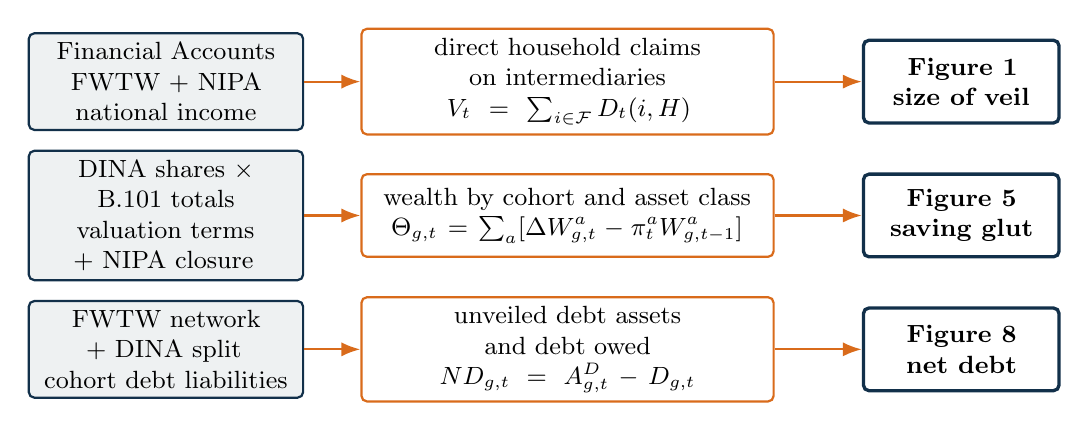
\begin{tikzpicture}[
    source/.style={draw=MSSNavy,thick,rounded corners=2pt,fill=MSSNavy!7,
      text width=3.25cm,minimum height=1.05cm,align=center,font=\small},
    object/.style={draw=MSSOrange,thick,rounded corners=2pt,fill=white,
      text width=5.0cm,minimum height=1.05cm,align=center,font=\small},
    result/.style={draw=MSSNavy,very thick,rounded corners=2pt,fill=white,
      text width=2.25cm,minimum height=1.05cm,align=center,font=\small\bfseries},
    arrow/.style={-{Latex[length=2.4mm]},thick,color=MSSOrange}
  ]
    \node[source] (s1) at (0,3.4)
      {Financial Accounts\\FWTW + NIPA national income};
    \node[object] (o1) at (5.1,3.4)
      {direct household claims on intermediaries\\
       \(V_t=\sum_{i\in\mathcal F}D_t(i,H)\)};
    \node[result] (r1) at (10.1,3.4) {Figure 1\\size of veil};

    \node[source] (s2) at (0,1.7)
      {DINA shares \(\times\) B.101 totals\\valuation terms + NIPA closure};
    \node[object] (o2) at (5.1,1.7)
      {wealth by cohort and asset class\\
       \(\Theta_{g,t}=\sum_a[\Delta W^a_{g,t}
       -\pi^a_tW^a_{g,t-1}]\)};
    \node[result] (r2) at (10.1,1.7) {Figure 5\\saving glut};

    \node[source] (s3) at (0,0)
      {FWTW network + DINA split\\cohort debt liabilities};
    \node[object] (o3) at (5.1,0)
      {unveiled debt assets\\and debt owed\\
       \(ND_{g,t}=A^D_{g,t}-D_{g,t}\)};
    \node[result] (r3) at (10.1,0) {Figure 8\\net debt};

    \draw[arrow] (s1) -- (o1); \draw[arrow] (o1) -- (r1);
    \draw[arrow] (s2) -- (o2); \draw[arrow] (o2) -- (r2);
    \draw[arrow] (s3) -- (o3); \draw[arrow] (o3) -- (r3);
  \end{tikzpicture}
  \caption{Dataset roles in the three selected July 2025 exhibits.  DFA, the
    SCF panel, and income-minus-consumption estimates are validation layers,
    not substitutes for the baseline inputs.}
  \label{fig:data-flow}
\end{figure}

\subsection{The direct network is a Financial Accounts object}

For each of the \(\ell=34\) instruments, let \(X_{h,t}(i,j)\) be the dollar
stock issued by sector \(i\) and held by sector \(j\).  Financial Accounts
issuance and holding totals impose the margins

\begin{equation}
  r_{iht}=\sum_jX_{h,t}(i,j),
  \qquad
  c_{jht}=\sum_iX_{h,t}(i,j).
  \label{eq:fwtw-margins}
\end{equation}

Detailed Financial Accounts fields supply exact bilateral cells where they
are available.  If a margin contains exactly one unknown cell, that cell can
indeed be recovered as a simple residual.  With several unknown cells, however,
the margins do not identify a unique matrix.  The 2025 paper follows the Batty
et al. procedure: known relationships and exclusion restrictions are retained,
and the remaining cells are completed using proportionality and a balancing
algorithm that respects known row and column totals.  DINA does not enter this
completion.  After completing each \(X_{h,t}\), the paper constructs

\begin{equation}
  \matM_t
  =\operatorname{diag}(L_t)^{-1}\sum_{h=1}^{34}X_{h,t},
  \qquad \matM_t\mathbf 1=\mathbf 1,
  \label{eq:fwtw-to-direct}
\end{equation}

where \(L_{i,t}\) is total liabilities issued by sector \(i\).  Thus the
intuition that there are 23 instruments needs one dimensional correction:
the paper has 23 intermediary sectors, four ultimate-owner sectors, and 34
instrument matrices.

\subsection{DINA expands the household owner; it does not supply counterparties}

DINA is a tax-record-based distributional microfile.  The authors use it to
estimate

\begin{equation}
  \omega^a_{g,t}
  =\frac{\text{household wealth class \(a\) held by cohort \(g\)}}
         {\text{aggregate household wealth class \(a\)}},
  \qquad \sum_g\omega^a_{g,t}=1.
  \label{eq:dina-share}
\end{equation}

For the saving calculation, these shares distribute the corresponding
Financial Accounts B.101 total:

\begin{equation}
  W^a_{g,t}=\omega^a_{g,t}W^a_t.
  \label{eq:dina-times-b101}
\end{equation}

For distributional unveiling, Appendix Table A1 maps each Financial Accounts
instrument \(h\) to a broad DINA asset class \(a(h)\).  Operationally, a direct
household position can then be split into cohort columns as

\begin{equation}
  X^{\mathrm{aug}}_{h,t}(i,g)
  =X_{h,t}(i,H)\omega^{a(h)}_{g,t}.
  \label{eq:augmented-household-column}
\end{equation}

The unveiling is repeated on the augmented matrix.  Consequently, DINA is not
a dataset of observed
\((\text{wealth group},\text{intermediary},\text{instrument})\) counterparties.
It supplies group shares for mapped household asset and liability classes.
Combining those shares with Financial Accounts totals creates the
distributional columns.

\subsection{How the selected figures use the layers}

\begin{table}[htbp]
  \centering
  \caption{Main datasets and their economic roles}
  \label{tab:main-data-roles}
  \small
  \begin{tabular}{@{}
    >{\raggedright\arraybackslash}p{0.21\textwidth}
    >{\raggedright\arraybackslash}p{0.25\textwidth}
    >{\raggedright\arraybackslash}p{0.44\textwidth}@{}}
    \toprule
    \textbf{Source} & \textbf{Observed object} & \textbf{Role in this project} \\
    \midrule
    Financial Accounts / FWTW
      & Sector--instrument stocks; issuer--holder positions; B.101 household
        balance sheet
      & Builds \(X_{h,t}\), \(\matM_t\), and \(\Omega_t\).  It identifies
        Figure 1's aggregate amount behind the veil and the primary assets
        used in Figure 8. \\
    DINA (\code{PSZusdina})
      & Individual tax-record-based income and imputed wealth components,
        collapsed to cohort--asset shares
      & Baseline distribution of B.101 wealth for Figure 5; splits the
        household owner into wealth cohorts for Figure 8.  It is not needed
        for aggregate Figure 1. \\
    NIPA
      & Aggregate national income, disposable income, consumption, personal
        and corporate saving
      & Gives Figure 1's national-income denominator and forces
        distributional saving in Figure 5 to aggregate to national-account
        private saving. \\
    JST and debt write-down inputs
      & House-price appreciation; write-down rates by debt type and group
      & Identify pure valuation terms \(\pi^a_t\).  Equity price inflation is
        the residual that closes aggregate wealth-based saving to NIPA. \\
    DFA and SCF panel
      & Alternative wealth shares; 1983--1989 household wealth panel
      & Validate DINA wealth shares and repeated-cross-section saving
        estimates. \\
    SCF consumption, CEX, and PSID
      & Survey expenditures, income, and household characteristics
      & Support the Appendix C.1 income-minus-consumption robustness exercise;
        CEX and PSID do not represent the richest households well enough to be
        the 2025 baseline. \\
    \bottomrule
  \end{tabular}
\end{table}

Figure 1 therefore needs the Financial Accounts/FWTW network and NIPA only for
the \(NI_t\) normalization; neither DINA nor consumption microdata are required.
Figure 5 instead uses the wealth-based identity

\begin{equation}
  \Theta_{g,t}
  =\sum_a\left[
    W^a_{g,t}-W^a_{g,t-1}-\pi^a_tW^a_{g,t-1}
  \right].
  \label{eq:distributional-saving}
\end{equation}

Here \(\pi^a_t\) is pure asset-price inflation, not the total return.  The JST
repeat-sales house-price index identifies housing valuation, fixed-income
price inflation is zero under the Financial Accounts convention, debt
write-downs are treated as borrower valuation gains, and equity inflation is
chosen residually so that \(\sum_g\Theta_{g,t}\) matches total private saving
in NIPA.

Income less consumption,
\(\Theta_{g,t}=Z_{g,t}-T_{g,t}+R_{g,t}-C_{g,t}\), is a separate robustness
method in Appendix C.1.  DINA supplies pre-tax income, taxes, and transfers;
the authors use SCF-based consumption shares and CEX evidence to scale the
observed consumption categories.  The paper explicitly cautions that CEX and
PSID do not measure consumption at the very top accurately.  It is therefore
incorrect to describe CEX or PSID as the baseline route to Figure 5.

Finally, Figure 8 uses the augmented unveiling result
\(A_t=P_t\Omega_t+\Lambda_t\).  If \(A^D_{g,t}\) is household debt held as an
asset by cohort \(g\) and \(D_{g,t}\) is debt owed by that cohort, then
\(ND_{g,t}=A^D_{g,t}-D_{g,t}\).  The asset side requires the unveiled FWTW
network; both the asset and liability sides require the household cohort
mapping.  NIPA enters only when the resulting stocks are normalized by
national income.

\section{Comparison with the authors' 2021 implementation}
\label{sec:comparison}

\subsection{Version boundary}

The available replication package is for the February 2021 paper, whereas the
target article is the heavily revised July 2025 draft. The 2021 Stata code does
not create the 2025 paper's $27\times27$ completed ownership matrix and does not
evaluate Equation~\eqref{eq:paper-leontief}. Instead,
\path{MSS2021Febreplicationkit/code/build_fa_unveiling_data.do} allocates
household debt, government debt, and mortgage debt through separate,
instrument-specific sequences.

For household debt, round 1 identifies the direct holders and checks their sum
with \code{test1} (lines 131 and 166--171). Subsequent round markers occur at
lines 724, 1066, 1259, 1740, 2138, and 2316. At each stage the script passes
the debt embedded in selected intermediary assets to the holders of those
intermediaries' liabilities. The final stage constructs owner and residual
categories at lines 2385--2388 and saves \code{Yunveilhhd.dta} at line 2405.
Government and mortgage debt repeat the procedure in separate code blocks.

\begin{table}[htbp]
  \centering
  \caption{The two implementations solve related, but not identical, empirical
    problems.}
  \label{tab:implementation-comparison}
  \small
  \begin{tabular}{@{}p{0.19\textwidth}p{0.36\textwidth}p{0.36\textwidth}@{}}
    \toprule
     & \textbf{2025 paper and our Python}                                            & \textbf{February 2021 Stata package} \\
    \midrule
    Representation
     & One completed direct-ownership matrix $\matM_t$
     & Instrument- and sector-specific dollar variables                                                                     \\
    Recursion
     & The same $B_t,Q_t$ operate at every path length
     & Different instruments and sector rules are opened at named stages                                                    \\
    Stopping rule
     & Exact infinite sum when $\rho(Q_t)<1$
     & Seven economically ordered stages plus residual buckets                                                              \\
    Data treatment
     & Completed FWTW cells are an upstream input
     & Proportionality factors, net issuance, and special cases are coded inline                                            \\
    Conservation
     & Owner shares sum to one
     & \code{test1}--\code{test7} preserve the relevant debt stock                                                          \\
    Output
     & Share matrices $\Omega_t$ and $A_t$
     & Dollar totals assigned to household, government, foreign, and residual owners                                        \\
    \bottomrule
  \end{tabular}
\end{table}

\subsection{What can be proved to be the same}

Suppose an explicit round-by-round algorithm is applied to the same fixed
$B_t,Q_t$ used by the matrix method. After $R$ rounds it produces

\begin{equation}
  \Omega_t^{(R)}=\sum_{r=0}^{R-1}Q_t^rB_t.
\end{equation}

If $\rho(Q_t)<1$, the finite sequence converges to the Leontief solution:

\begin{equation}
  \lim_{R\rightarrow\infty}\Omega_t^{(R)}
  =(I-Q_t)^{-1}B_t=\Omega_t.
\end{equation}

The remaining truncation error has the exact expression

\begin{equation}
  \Omega_t-\Omega_t^{(R)}=Q_t^R\Omega_t.
  \label{eq:truncation-error}
\end{equation}

This establishes algebraic equivalence between a stationary round algorithm
and our linear solve. In the worked example, seven terms have a maximum error
of \ToyMaxSevenRoundGap{} in ownership shares, or
\ToyMaxSevenRoundGapPP{} percentage points. The 80-term test agrees with the
closed form to an absolute tolerance of $10^{-12}$.

This numerical exercise must not be confused with running the actual seven
rounds in the authors' Stata file. Their stages are not seven powers of one
fixed $Q_t$: they unveil different instruments, alter sector treatments, use
net-issuance adjustments, and retain explicitly defined residuals. Equation
\eqref{eq:truncation-error} therefore proves the common mathematical principle,
not equality of the two historical empirical pipelines.

\subsection{Evidentiary conclusion}

The present evidence supports three deliberately bounded conclusions.

\begin{enumerate}
  \item \textbf{Exact algebraic consistency with the 2025 paper.} Our block
        solve is the lower-left block of the paper's Equation~(1), and the unit
        tests establish numerical equality on a common matrix.
  \item \textbf{Conceptual consistency with the 2021 package.} Both methods
        recursively attribute an intermediary's embedded assets according to the
        ownership of its liabilities, while preserving the total amount being
        allocated.
  \item \textbf{No completed empirical equality test across versions.} The
        2021 package and 2025 exposition differ in inputs, instruments, sector
        definitions, residual treatment, and sample period. The completed 2025
        annual matrices are not included in the old package.
\end{enumerate}

It would therefore be incorrect at this stage to claim either that the two
actual implementations lead to the same empirical series or that a difference
shows an error in the paper. Nor is the Python method unconditionally
``better.'' It is shorter, numerically exact for the stationary operator, and
closer to the 2025 exposition. The Stata implementation is more explicit about
the instrument-specific empirical adjustments used in the earlier paper.
Those are different strengths attached to different versions of the research
design.

\subsection{Protocol for the eventual numerical comparison}

A defensible empirical comparison requires a common-input experiment:

\begin{enumerate}
  \item construct the same completed issuer--holder dollar matrices and sector
        aggregation for both algorithms;
  \item derive $B_t$ and $Q_t$ and run the Python Leontief solve;
  \item reproduce the authors' relevant allocation rules in an isolated copy
        of the Stata pipeline, preserving its residual definitions;
  \item aggregate both outputs to identical owner, asset, date, and unit
        definitions;
  \item compare cell-level and aggregate differences using a predeclared
        maximum absolute share tolerance and verify total-debt conservation; and
  \item attribute any remaining discrepancy to truncation, residual treatment,
        missing-cell completion, net issuance, or a genuine coding difference.
\end{enumerate}

Only after this protocol can the report make a supported statement about
numerical equality. A claim that the paper is partially wrong would require a
reproducible violation of its stated equations or accounting identities on the
authors' own intended inputs, not merely a difference from the older package.

\section{Reconstruction of Figure 1}
\label{sec:figure1}

\subsection{What the figure measures}

Figure 1 measures the size of the balance-sheet layer that must be unveiled.
Let $D_t(i,H)$ be the dollar liabilities issued by sector $i$ and held by the
household sector, after summing the FWTW cells over instruments. If
$\mathcal F$ is the set of financial-intermediary issuers, define

\begin{equation}
  V_t=\sum_{i\in\mathcal F}D_t(i,H).
  \label{eq:figure1-veil}
\end{equation}

The household's claim in Equation~\eqref{eq:figure1-veil} is direct with
respect to the intermediary but indirect with respect to the primary assets
that the intermediary finances. This is why it is the amount that ``needs to
be unveiled.'' It is not the elementwise difference between $\Omega_t$ and
$\matM_t$, which have different dimensions and economic meanings. The paper
plots

\begin{equation}
  \frac{V_t}{\sum_{i\ne ROW}D_t(i,H)}
  \qquad\text{and}\qquad
  \frac{V_t}{NI_t},
  \label{eq:figure1-series}
\end{equation}

where the first denominator is household holdings of U.S. financial assets
and $NI_t$ is annual national income. Both balance-sheet amounts are Q4 stocks
in current dollars; national income is a current-dollar annual flow.

\subsection{Three evidence layers}

The empirical exercise must distinguish three questions.  First, the
February 2021 package can be run on its own final files to benchmark the older
paper, but that package has no predecessor of the revised Figure~1.  Second,
we can reconstruct the Figure~1 numerator from the authors' supplied source
vintage.  Third, the June 2026 public FWTW release provides a new-data
robustness exercise.  The third layer cannot substitute for the second.

The 2025 article uses $k=23$ intermediary sectors and $\ell=34$ financial
instruments.  These numbers must not be conflated: there are 23 sectors, not
23 instruments.  The February 2021 package explicitly says that its prepared
\code{LQpanel\_2019Q1.dta} omits the underlying FWTW text files.  It therefore
does not contain the completed $34$ instrument matrices used by the July 2025
paper.  The link labelled ``replication kit'' in the supplied 2025 PDF also
resolves to the placeholder \code{NEW LINK.pdf}, so it does not supply the
missing vintage.

\subsection{Authors-data reconstruction from the February 2021 snapshot}

We start from the following prepared inputs rather than rerunning every
upstream import and merge:

\begin{itemize}
  \item \code{LQpanel\_2019Q1.dta}: the authors' quarterly wide Financial
        Accounts panel; we select Q4 stocks and the required household
        instruments;
  \item \code{Yunveilhhd.dta}: only the authors' already-computed allocation
        of aggregate corporate bonds to ABS issuers, finance companies,
        mortgage REITs, and depository institutions;
  \item \code{msf.dta}: the supplied licensed CRSP monthly security file,
        from which we construct the corporate-equity extension; and
  \item \code{YinequalityNIPAanalysis.dta}: the authors' annual national
        income series, which fixes the common-input sample at 1963--2016.
\end{itemize}

This skips mechanical source ingestion, table cleaning, and merges that the
authors have already performed.  It does \emph{not} skip the economically
central aggregation.  Our code constructs

\begin{align}
  V_t^{A}={}&C_t+T_t+MMF_t+GSE_t+MF_t+LI_t
    +(PE_t-UPE_t) \notag\\
    &+FB_t+FE_t,
  \label{eq:authors-figure1-sum}
\end{align}

where the terms denote checkable deposits and currency, time and saving
deposits, money-market-fund shares, GSE securities, mutual-fund shares, life
insurance reserves, funded pension entitlements, financial-intermediary bonds,
and listed financial-intermediary equity.  These are the nine nonzero
household-intermediary claim groups recoverable from the old snapshot.  The
remaining paper instruments either represent direct primary claims, have no
household position in this vintage, or require the missing bilateral FWTW
cells.  Every component in Equation~\eqref{eq:authors-figure1-sum} remains in
the generated annual data, and the code verifies that their sum equals
$V_t^{A}$.

For the equity extension, we retain December CRSP observations, reproduce the
authors' exclusion of foreign-incorporated share codes, and classify SIC
6000--6399 and 6700--6799 as listed financial intermediaries.  Prices times
shares outstanding are converted to millions of dollars.  We then apply the
old paper's proportionality logic,

\begin{equation}
  FE_t=
  \frac{\text{household corporate-equity assets}_t}
       {\text{all corporate-equity assets}_t}
  \times
  \text{listed financial market capitalization}_t.
  \label{eq:authors-equity-extension}
\end{equation}

The implementation is
\path{Code/unveiling/figure1_authors.py}; the thin entry point is
\path{Code/scripts/build_figure1_authors_data.py}.  Four tests check the
component identity, unit conversion, denominator exclusions, and annual merge
contract.

\subsection{The level is closely reproduced; the share denominator is not}

We digitize the two colored lines from the raster embedded on physical PDF
page 11.  The digitization is a generated, approximate benchmark, independent
of the reconstruction.  A few pixels of line thickness imply approximately
two percentage points of national income on the left axis and less than one
percentage point on the right axis.

\begin{figure}[htbp]
  \centering
  \includegraphics[width=\textwidth]{../Results_Proposal/figures/figure1_authors_data_comparison.png}
  \caption{Figure 1 benchmark and reconstruction from the authors' February
    2021 source vintage.  The left panel is directly comparable.  The two
    right-panel denominators diagnose the missing 2025 FWTW boundary.}
  \label{fig:figure1-authors-comparison}
\end{figure}

\begin{table}[htbp]
  \centering
  \caption{Quantitative authors-data comparison, 1963--2016}
  \label{tab:figure1-authors-comparison}
  \small
  \begin{tabular}{@{}p{0.42\textwidth}p{0.24\textwidth}p{0.24\textwidth}@{}}
    \toprule
    \textbf{Statistic} & \textbf{2025 figure, digitized} &
      \textbf{Our reconstruction} \\
    \midrule
    Level in \AuthorFigureStartYear
      & \PaperDigitizedStartLevel & \AuthorFigureStartLevel \\
    Level in \AuthorFigureEndYear
      & \PaperDigitizedEndLevel & \AuthorFigureEndLevel \\
    Annual level MAE
      & \multicolumn{2}{c}{\AuthorFigureLevelMAE} \\
    Annual level correlation
      & \multicolumn{2}{c}{\AuthorFigureLevelCorrelation} \\
    Share MAE, broad balance-sheet denominator
      & \multicolumn{2}{c}{\AuthorFigureShareBroadMAE} \\
    Share MAE, old-kit paper-scope proxy
      & \multicolumn{2}{c}{\AuthorFigureShareProxyMAE} \\
    \bottomrule
  \end{tabular}
\end{table}

The left-axis result is strong: the reconstructed level has an annual
correlation of \AuthorFigureLevelCorrelation{} with the plotted line and an
MAE of \AuthorFigureLevelMAE{} of national income.  It starts at
\AuthorFigureStartLevel{} rather than \PaperDigitizedStartLevel{} and reaches
\AuthorFigureEndLevel{} rather than \PaperDigitizedEndLevel{}.  Thus the
authors' older source data plus the explicit equity extension recover almost
all of the plotted stock behind the veil.

The right-axis result is less definitive because its exact denominator needs
the missing completed issuer--holder matrix.  A broad funded household
balance-sheet denominator is closer to the plotted series
(MAE \AuthorFigureShareBroadMAE{}) than the old kit's available implementation
of the paper's stated nonfinancial/foreign/residual exclusions
(MAE \AuthorFigureShareProxyMAE{}).  This ordering is evidence of a versioned
measurement boundary, not a license to choose the denominator with the lower
error.  The paper-scope proxy relies on older proportional allocations that
are not the Batty et al. completion algorithm adopted in 2025.

\subsection{New-data robustness remains a separate result}

The June 2026 public FWTW reconstruction remains informative.  It produces
\FigureOneStartShare{} in \FigureOneStartYear{}, \FigureOneSevenShare{} in
2007, a peak of \FigureOnePeakShare{} in \FigureOnePeakYear{}, and
\FigureOneEndShare{} in 2019.  Its level rises from \FigureOneStartLevel{} to
\FigureOneEndLevel{}.  This later-vintage result follows the central trend,
but it is not the same-input replication because it uses 21 rather than 23
intermediary definitions and later Financial Accounts revisions.

The defensible conclusion is therefore asymmetric.  We have a close
close old-vintage authors-data reproduction of Figure~1's level and a robust newer-data share
pattern.  We do not yet have the exact 2025 share denominator or completed
annual matrices.  No result here shows that the paper is wrong; making that
claim would require the missing intended inputs and a reproducible failure of
their stated identities.

\enlargethispage{2\baselineskip}
\section*{Sources and reproducibility}

The authoritative methodological source is Mian, Straub, and Sufi,
\emph{The Saving Glut of the Rich}, July
25, 2025 draft, Sections 2.1--2.2. The historical implementation source is the
read-only February 2021 replication package, especially
\path{MSS2021Febreplicationkit/code/build_fa_unveiling_data.do}. Project
notation, code contracts, exact line crosswalks, and the current empirical
boundary are documented in \path{docs/methods/leontief-unveiling.md},
\path{docs/data/figure1-data.md}, and
\path{docs/reference/author-kit-map.md}. Numerical values in this report are
generated by \path{Code/scripts/build_unveiling_teaching_assets.py},
\path{Code/scripts/build_figure1.py}, and
\path{Code/scripts/build_figure1_authors_data.py}.

\end{document}
